% =====================================================================
% MTH321 Numerical Analysis of Partial Differential Equations
% Project 2: Finite Difference Solution of a Poisson Problem with
% Mixed Boundary Data (Direction 2)
% Beamer slides; 4:3; compiles with pdflatex.
% Compile TWICE (frame counter "n / N" and the top bar need 2 runs).
% Missing figures are replaced by a purple "TODO figure" box, so the
% file always compiles. Edit \figdir and the file names below.
% =====================================================================
\documentclass[aspectratio=43]{beamer}

\usepackage[utf8]{inputenc}
\usepackage[T1]{fontenc}
\usepackage{lmodern}
\usepackage{amsmath,amssymb,amsfonts}
\usepackage{mathtools}
\usepackage{booktabs}
\usepackage{etoolbox}
\usepackage{appendixnumberbeamer}
\usepackage{tikz}
\usepackage{pgfplots}
\pgfplotsset{compat=1.17}
\usepgfplotslibrary{groupplots}
\usetikzlibrary{arrows.meta,calc,positioning}

% ---------------- colours (template W01) ----------------
\definecolor{rblue}{RGB}{51,51,170}
\definecolor{ralert}{RGB}{153,51,153}
\setbeamercolor{structure}{fg=rblue}
\setbeamercolor{alerted text}{fg=ralert}
\setbeamercolor{section in head/foot}{parent=structure,bg=white,fg=rblue}
\setbeamercolor{mini frame}{parent=structure}

% ---------------- outer theme: miniframes (top index bar) ----------------
\useoutertheme[subsection=false]{miniframes}
\setbeamerfont{section in head/foot}{size=\tiny}
\setbeamercolor{headline separator}{bg=rblue}

\setbeamertemplate{headline}{%
  \leavevmode%
  \begin{beamercolorbox}[wd=\paperwidth]{section in head/foot}
    \vskip2pt
    \insertnavigation{\paperwidth}%
    \vskip2pt%
  \end{beamercolorbox}%
  \begin{beamercolorbox}[wd=\paperwidth,ht=3pt,dp=0pt]{headline separator}
    \rule{\paperwidth}{3pt}%
  \end{beamercolorbox}%
}

% ---------------- footline: frame number only ----------------
\setbeamertemplate{footline}{%
  \hbox to\paperwidth{\hfil\usebeamerfont{footline}\color{black!50}%
  \insertframenumber\ /\ \inserttotalframenumber\hspace*{2mm}}%
  \vskip1pt%
}

\setbeamertemplate{frametitle}[default][center]

\setbeamertemplate{itemize item}{\textcolor{rblue}{\large\textbullet}}
\setbeamertemplate{itemize subitem}{\textcolor{rblue}{\normalsize\textbullet}}
\setbeamertemplate{itemize subsubitem}{\textcolor{rblue}{\small\textbullet}}
\setbeamertemplate{itemize/enumerate body begin}{\setlength{\itemsep}{0.45ex}\setlength{\parskip}{0pt}}
\setbeamertemplate{itemize/enumerate subbody begin}{\setlength{\itemsep}{0.3ex}\setlength{\parskip}{0pt}}
\setbeamertemplate{itemize/enumerate subsubbody begin}{\setlength{\itemsep}{0.2ex}\setlength{\parskip}{0pt}}

\setbeamertemplate{section in toc}{%
  \par\smallskip{\color{rblue}\textbullet}\ \textbf{\inserttocsection}\par}
\setbeamertemplate{navigation symbols}{}

\newcommand{\bb}[1]{{\color{rblue}\bfseries #1}}
\newcommand{\figcap}[1]{\par\vspace{2pt}{\centering\small #1\par}}

% ---------------- extra styling ----------------
\definecolor{rlight}{RGB}{236,238,250}
\definecolor{rgrey}{RGB}{95,95,115}
\setbeamertemplate{blocks}[rounded][shadow=false]
\setbeamercolor{block title}{bg=rblue,fg=white}
\setbeamercolor{block body}{bg=rlight,fg=black}
% one-line message of every frame (same colours as the block titles)
\newcommand{\takeaway}[1]{\par\vfill%
  \begin{beamercolorbox}[wd=\linewidth,rounded=true,sep=4pt]{block title}%
  \small\textbf{Takeaway.}\ #1%
  \end{beamercolorbox}\vskip1pt}
\newcommand{\chip}[2]{\tikz[baseline=-0.6ex]\node[chip=#1]{#2};}
\tikzset{
  card/.style={draw=rblue!45, fill=rlight, rounded corners=4pt, line width=0.6pt},
  chip/.style={draw=#1, fill=#1!12, text=#1!75!black, rounded corners=2pt,
               inner sep=2.5pt, font=\scriptsize\bfseries, anchor=west},
  num/.style={circle, fill=rblue, text=white, font=\scriptsize\bfseries, inner sep=1.8pt}
}

% ---------------- figures: folder + safe include ----------------
% \figdir: folder holding the PNG/PDF files (relative to this .tex).
% \fig{file}{fraction of \linewidth}: includes the file if it exists,
% otherwise draws a placeholder box (so the document always compiles).
\newcommand{\figdir}{../figures/}
\newcommand{\fig}[2]{%
  \IfFileExists{\figdir #1}%
    {\includegraphics[width=#2\linewidth]{\figdir #1}}%
    {\fbox{\parbox[c][2.6cm][c]{#2\linewidth}{\centering\scriptsize\color{ralert}
      TODO figure:\\[2pt] \detokenize{#1}}}}}

% fixed-HEIGHT figure include (for tall figures); #2 = fraction of \textheight
\newcommand{\figh}[2]{%
  \IfFileExists{\figdir #1}%
    {\includegraphics[height=#2\textheight,keepaspectratio]{\figdir #1}}%
    {\fbox{\parbox[c][#2\textheight][c]{0.4\linewidth}{\centering\scriptsize\color{ralert}
      TODO figure:\\[2pt] \detokenize{#1}}}}}





\begin{document}

% =====================================================================
% 1. Title
% =====================================================================
\newcommand{\member}[2]{\parbox[t]{3.3cm}{\centering\small #1\\[1pt]{\scriptsize\color{black!55} #2}}}
\begin{frame}
\centering
\vfill
{\scriptsize\color{black!55}\textsc{MTH321 \;$\cdot$\; Numerical Analysis of Partial Differential Equations}\par}
\vskip14pt
{\color{rblue}\Large\bfseries Finite Difference Solution of a Poisson\\[3pt] Problem with Mixed Boundary Data\par}
\vskip6pt
{\small\color{black!70} Does the right-edge closure decide the accuracy?\par}
\vskip24pt
\member{Rengerile Na}{2359838}\hspace{0.3cm}\member{Suning Peng}{2361786}\hspace{0.3cm}\member{Kainan Zhao}{2362073}\\[8pt]

\vspace{15pt}
\vfill
{\footnotesize\color{black!70} Xi'an Jiaotong-Liverpool University\\[2pt]
\scriptsize October 2026\par}
\vfill
\end{frame}

% =====================================================================
% 2. Roadmap  (before the first \section: no dot in the top bar)
% =====================================================================


\begin{frame}{Presentation Roadmap}
\centering

% Research question: smaller and closer to the title
\vspace{-15pt}

{\normalsize
How does the \bb{right-edge boundary row} affect\\[3pt]
accuracy, matrix structure and computational cost?
}

% Four stages: centered in the available slide area
\vspace{0.75cm}

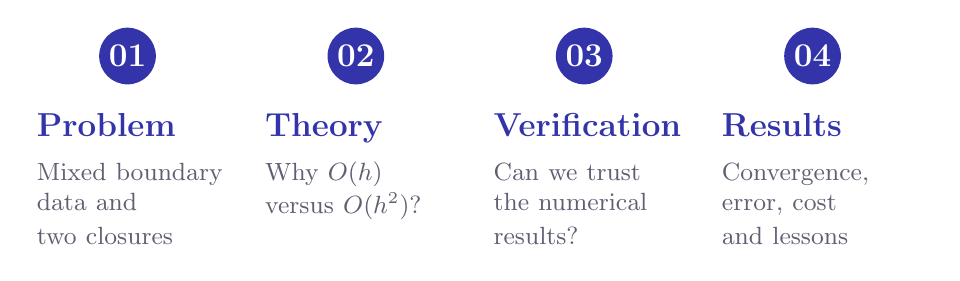
\begin{tikzpicture}[x=1cm,y=1cm]

% Centers of the four columns
\def\xA{-4.35}
\def\xB{-1.45}
\def\xC{1.45}
\def\xD{4.35}

% Numbered circles
\foreach \x/\n in {
    \xA/01,
    \xB/02,
    \xC/03,
    \xD/04
}{
    \node[
        circle,
        fill=rblue,
        text=white,
        minimum size=0.72cm,
        inner sep=0pt,
        font=\large\bfseries
    ] at (\x,0.65) {\n};
}

% Stage 1
\node[
    anchor=north west,
    text width=2.55cm,
    align=left
] at (\xA-1.275,0.05) {
    {\large\bfseries\color{rblue}Problem}\\[5pt]
    {\small\color{rgrey}
    Mixed boundary data and\\
    two closures}
};

% Stage 2
\node[
    anchor=north west,
    text width=2.55cm,
    align=left
] at (\xB-1.275,0.05) {
    {\large\bfseries\color{rblue}Theory}\\[5pt]
    {\small\color{rgrey}
    Why $O(h)$ \\versus
    $O(h^2)$?}
};

% Stage 3
\node[
    anchor=north west,
    text width=2.55cm,
    align=left
] at (\xC-1.275,0.05) {
    {\large\bfseries\color{rblue}Verification}\\[5pt]
    {\small\color{rgrey}
    Can we trust \\the
    numerical\\ results?}
};

% Stage 4
\node[
    anchor=north west,
    text width=2.55cm,
    align=left
] at (\xD-1.275,0.05) {
    {\large\bfseries\color{rblue}Results}\\[5pt]
    {\small\color{rgrey}
    Convergence, error, cost\\
    and lessons}
};

\end{tikzpicture}

\vfill

\end{frame}

% =====================================================================
\section[Problem \& Methods]{Problem \& Methods}
% =====================================================================

% ---------------- 3. Why mixed data? ----------------
\begin{frame}{Why Do Boundary Rows Matter?}
\begin{columns}[T]
\column{0.42\linewidth}
\centering
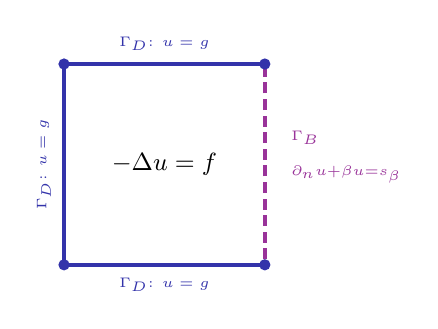
\begin{tikzpicture}[scale=0.85]
  \draw[rblue, line width=1.6pt] (0,0) -- (0,3) (0,0) -- (3,0) (0,3) -- (3,3);
  \draw[ralert, line width=1.6pt, dash pattern=on 4pt off 2pt] (3,0.08) -- (3,2.92);
  \foreach \p in {(0,0),(0,3),(3,0),(3,3)} \fill[rblue] \p circle (2.4pt);
  \node at (1.5,1.5) {\small $-\Delta u=f$};
  \node[rblue, font=\tiny] at (1.5,-0.3) {$\Gamma_D$: $u=g$};
  \node[rblue, font=\tiny] at (1.5,3.3) {$\Gamma_D$: $u=g$};
  \node[rblue, font=\tiny, rotate=90] at (-0.3,1.5) {$\Gamma_D$: $u=g$};
  \node[ralert, font=\tiny, align=center, anchor=west] at (3.25,1.9) {$\Gamma_B$};
  \node[ralert, font=\tiny, align=center, anchor=west] at (3.25,1.35) {$\partial_n u{+}\beta u{=}s_\beta$};
\end{tikzpicture}
\column{0.56\linewidth}
\small
\begin{itemize}
\item \bb{Neumann} ($\beta=0$): prescribed flux; insulated edge if $q=0$
\item \bb{Robin} ($\beta=\mathrm{Bi}=HL/k$): convection to a fluid; $\beta=2$ means $\mathrm{Bi}=2$
\item \bb{Benchmark} $u^\ast=e^{x+y}$: exact data, so the error is known
\end{itemize}
\end{columns}
{\small Same five-point interior stencil --- only the \alert{right-edge row} is a modelling choice.}
\takeaway{Real boundaries mix values, fluxes and convection; the closure is part of the method, so we test it.}
\end{frame}

% ---------------- 4. Two closures ----------------

\begin{frame}{Two Right-Edge Closures}

\begin{columns}[T,onlytextwidth]

% Left column: FO closure
\column{0.47\textwidth}

\begin{beamercolorbox}[wd=\linewidth,rounded=true,sep=3pt]{block title}
\small\textbf{FO: derivative row}
\end{beamercolorbox}

\begin{beamercolorbox}[wd=\linewidth,rounded=true,sep=4pt]{block body}
\begin{minipage}[t][3.85cm][t]{\linewidth}
\footnotesize

Backward difference \bb{replaces} the PDE row:

\[
\Big(\frac1h+\beta\Big)U_{N,j}
-\frac1h U_{N-1,j}=s_{\beta,j}
\]

\vfill

{\small No tangential coupling}

\vspace{0.1cm}

Boundary defect:
\(\displaystyle -\frac h2u_{xx}\)

\end{minipage}
\end{beamercolorbox}

% Right column: ghost-point closure
\column{0.47\textwidth}

\begin{beamercolorbox}[wd=\linewidth,rounded=true,sep=3pt]{block title}
\small\textbf{G: ghost point, PDE row kept}
\end{beamercolorbox}

\begin{beamercolorbox}[wd=\linewidth,rounded=true,sep=4pt]{block body}
\begin{minipage}[t][3.85cm][t]{\linewidth}
\footnotesize

Eliminate \(U_{N+1,j}\) (ghost):

\[
\begin{aligned}
\Big(\frac4{h^2}+\frac{2\beta}{h}\Big)U_{N,j}
&-\frac2{h^2}U_{N-1,j}\\[-2pt]
&-\frac{U_{N,j-1}+U_{N,j+1}}{h^2}\\[-2pt]
&=f+\frac{2s_\beta}{h}
\end{aligned}
\]

\vfill

Boundary defect:
\(\displaystyle +\frac h3u_{xxx}\)

\end{minipage}
\end{beamercolorbox}

\end{columns}

\vspace{0.15cm}

\begin{center}
{\scriptsize\color{rgrey}
Interior defect \(O(h^2)\)
\quad $\cdot$ \quad
Boundary defects \(O(h)\)
\quad $\cdot$ \quad
\(N(N-1)\) unknowns
}
\end{center}

\takeaway{FO imposes a derivative row, while G keeps the PDE row. Their global performance may differ because of stability.}

\end{frame}


% ---------------- 5. From equations to a solver ----------------
\begin{frame}{From Equations to a Solver}
\centering
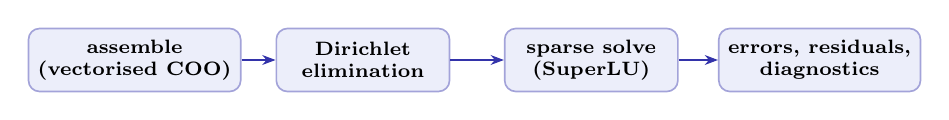
\begin{tikzpicture}[node distance=0.35cm, every node/.style={font=\scriptsize\bfseries}]
  \node[card, minimum width=2.2cm, minimum height=0.8cm, align=center] (a) at (0,0) {assemble\\(vectorised COO)};
  \node[card, minimum width=2.2cm, minimum height=0.8cm, align=center] (b) at (2.9,0) {Dirichlet\\elimination};
  \node[card, minimum width=2.2cm, minimum height=0.8cm, align=center] (c) at (5.8,0) {sparse solve\\(SuperLU)};
  \node[card, minimum width=2.2cm, minimum height=0.8cm, align=center] (d) at (8.7,0) {errors, residuals,\\diagnostics};
  \draw[-{Stealth}, rblue] (a) -- (b); \draw[-{Stealth}, rblue] (b) -- (c); \draw[-{Stealth}, rblue] (c) -- (d);
\end{tikzpicture}

\vspace{6pt}
\begin{columns}[T]
\column{0.52\linewidth}
\small
\begin{itemize}
\item Nonzeros: FO $(N-1)(5N-6)$, G $+\,2(N-2)$
\item Raw matrices are \bb{nonsymmetric}: $\|A-A^T\|_F/\|A\|_F=0.055$ at $N=32$
\item Weights $W$ (1 inside, $1/h$ for FO, $1/2$ for G) give $K=WA$ \bb{symmetric positive definite}
\end{itemize}
\column{0.52\linewidth}
\small
\begin{itemize}
\item Implemented by us: stencils, elimination, norms, weights
\item Delegated: SciPy sparse storage, SuperLU, GMRES, CG
\item \texttt{run\_all.py} regenerates every table and figure
\end{itemize}
\end{columns}
\takeaway{Nonsymmetry is not hidden by the self-adjoint PDE: CG applies only to the weighted system, which we prove SPD.}
\end{frame}

% =====================================================================
\section[Theory]{Theory}
% =====================================================================

% ---------------- 6. Why G gains a factor h ----------------
\begin{frame}{Why Does G Gain a Factor $h$?}
\small
\begin{center}
\begin{tabular}{@{}lccc@{}}
\toprule
 & boundary defect & stability estimate & max-norm error\\
\midrule
FO & $\tfrac{M_2}{2}h$ & $\|V\|_\infty\le\tfrac72(F_0+S_0)$ & $O(h)$\\
G  & $\tfrac{M_3}{3}h+\tfrac{M_4}{12}h^2$ & $\|V\|_\infty\le\tfrac74(2F_0+\textcolor{ralert}{h}S_0)$ & $O(h^2)$\\
\bottomrule
\end{tabular}
\end{center}
\vspace{2pt}
\begin{itemize}
\item Proof tools: \bb{discrete comparison principle} and the barrier $\psi=1+x-x^2/4$; the matrices are inverse positive
\item The estimate is uniform in $N$ and $\beta$: stability, not consistency, separates the two closures
\item Interior defect is $O(h^2)$ for both closures
\end{itemize}
\takeaway{G's $O(h)$ boundary defect enters the error multiplied by $h$; FO's does not, so FO is $O(h)$ and G is $O(h^2)$.}
\end{frame}

% ---------------- 7. From theory to testable predictions ----------------
\begin{frame}{From Theory to Testable Predictions}
\small
\begin{enumerate}
\item FO error $\Theta(h)$, G error $O(h^2)$, in the maximum and the discrete $L^2$ norm
\item The largest error sits on the \bb{right edge}
\item FO has a \bb{lower bound} $C_\beta h$ ($C_0=0.305$, $C_2=0.186$): first order is real, not just an upper bound
\end{enumerate}
\vspace{4pt}
\begin{center}
\footnotesize
\begin{tabular}{@{}lccc@{}}
\toprule
FO at $N=128$ & lower bound & measured & upper bound\\
\midrule
Neumann & $2.4\times10^{-3}$ & $6.9\times10^{-3}$ & $1.0\times10^{-1}$\\
Robin   & $1.5\times10^{-3}$ & $4.2\times10^{-3}$ & $1.0\times10^{-1}$\\
\bottomrule
\end{tabular}

\vspace{3pt}
The measured error lies between the bounds; the upper bound is conservative (15--24 times too large).
\end{center}
\takeaway{Theory gives predictions we can test; the lower bound shows FO's first order is genuine, not a weakness of the proof.}
\end{frame}

% =====================================================================
\section[Verification]{Verification}
% =====================================================================

% ---------------- 7. Four independent checks ----------------

\begin{frame}{Four Independent Checks of the Equations}
\small
\vspace{0.05cm}

\begin{columns}[T,onlytextwidth]

% Left column
\column{0.475\textwidth}

\begin{minipage}[t][1.95cm][t]{\linewidth}
{\normalsize\bfseries\color{rblue}1. Hand-derived row}\par
\vspace{0.08cm}
{\footnotesize For $N=4$, $j=1$: G row entries
$64+8\beta$, $-32$, $-16$.}\par
{\footnotesize Load: $(6+8\beta)e^{5/4}+16e$.}
\end{minipage}

\vspace{0.18cm}

\begin{minipage}[t][1.95cm][t]{\linewidth}
{\normalsize\bfseries\color{rblue}2. Polynomial defects}\par
\vspace{0.08cm}
{\footnotesize Test function: $u=1+x^3+y^4$.}\par
{\footnotesize $\tau_I=-2h^2$,
$\tau_{\rm FO}=-3h+h^2$,}\par
{\footnotesize $\tau_{\rm G}=2h-2h^2$.}
\end{minipage}

% Right column
\column{0.475\textwidth}

\begin{minipage}[t][1.95cm][t]{\linewidth}
{\normalsize\bfseries\color{rblue}3. Dense-system check}\par
\vspace{0.08cm}
{\footnotesize Uneliminated system: all Dirichlet
and ghost unknowns kept.}\par
{\footnotesize All 16 configurations agree to $10^{-11}$.}
\end{minipage}

\vspace{0.18cm}

\begin{minipage}[t][1.95cm][t]{\linewidth}
{\normalsize\bfseries\color{rblue}4. Independent P1 FEM}\par
\vspace{0.08cm}
{\footnotesize Independent reference: scikit-fem.}\par
{\footnotesize FEM error order: $2.00$.}\par
{\footnotesize FDM--FEM difference: 1.00 (FO),
2.00 (G).}
\end{minipage}

\end{columns}

\vspace{0.12cm}

\begin{center}
{\footnotesize\color{rgrey}
16 automated tests
 $\cdot$ 
Asymmetric test function catches $x\leftrightarrow y$ swaps.
}
\end{center}

\takeaway{Four independent checks agree: the assembled matrix matches the intended equations.}

\end{frame}


% ---------------- 8. Algebraic vs discretisation error ----------------
\begin{frame}{Is the Linear Solve Trustworthy?}
\begin{columns}[T]
\column{0.5\linewidth}
\centering
\fig{tolerance_sweep.png}{1.0}
\figcap{GMRES/direct difference relative to discretisation error ($N=64$); all below the 1\% line}
\column{0.56\linewidth}
\footnotesize
\begin{itemize}
\item Direct solve: componentwise residual $\le2.3\times10^{-12}$ over 24 runs
\item $\|A^{-1}\|_\infty$ stays in $[0.09,0.51]$ for all $h$; $\kappa_\infty\sim h^{-2}$
\item Estimated forward error $\le2.8\times10^{-6}$ of the discretisation error
\item ILU-GMRES and weighted CG agree: ratio $\le3.7\times10^{-5}$
\item Jacobi-GMRES at rtol $10^{-8}$ \alert{fails} for G ($7.4\times10^{-2}$); passes at $10^{-10}$
\end{itemize}
\end{columns}
\takeaway{Solver error is far below discretisation error, but the stopping tolerance must be chosen per closure: G needs a stricter one.}
\end{frame}

% =====================================================================
\section[Results]{Results}
% =====================================================================

% ---------------- 9. First vs second order ----------------
\begin{frame}{First Versus Second Order}
\centering
\fig{convergence.png}{0.98}

\vspace{2pt}
\footnotesize
\begin{tabular}{@{}lcccc@{}}
\toprule
 & FO $p_\infty$ & G $p_\infty$ & $E_\infty$(FO) at $h=\tfrac1{512}$ & $E_\infty$(G)\\
\midrule
Neumann & 1.005 & 2.000 & $1.7\times10^{-3}$ & $8.5\times10^{-7}$\\
Robin   & 1.003 & 2.000 & $1.0\times10^{-3}$ & $5.2\times10^{-7}$\\
\bottomrule
\end{tabular}
\takeaway{FO converges at order 1.00 and G at 2.00; at $h=1/512$ G is about 2000 times more accurate with only 0.08\% more nonzeros.}
\end{frame}

% ---------------- 10. Where does the error live? ----------------
\begin{frame}{Where Does the Error Live?}
\begin{columns}[T]
\column{0.58\linewidth}
\centering
\fig{boundary_vs_interior.png}{1.0}
\figcap{Maximum error on the right edge and in the interior}
\column{0.5\linewidth}
\footnotesize
\begin{itemize}
\item Global maximum = \bb{right-edge} maximum in every run
\item FO interior order $\approx1$: the boundary defect pollutes the whole field
\item G interior fit $1.98$; pairwise orders rise from $1.8$ to $1.99$ as the maximiser moves to $x=1$
\end{itemize}
\end{columns}
\takeaway{A second-order interior stencil does not give a second-order solution: the boundary row limits global accuracy.}
\end{frame}

% ---------------- 11. Cost at fixed accuracy ----------------
\begin{frame}{What Does the Accuracy Cost?}
\begin{columns}[T]
\column{0.52\linewidth}
\centering
\fig{cost_vs_accuracy.png}{1.0}
\figcap{Assembly plus solve time versus nodal error ($N=4,\dots,512$)}
\column{0.52\linewidth}
\footnotesize
\begin{itemize}
\item Targets $5\times10^{-3}\dots10^{-5}$: FO reaches only the two loosest within $N\le512$
\item Target $2\times10^{-3}$ (Neumann): FO needs $N=512$ ($\approx2.0$ s), G needs $N=16$ ($\approx1$ ms)
\item At equal $N=512$ the cost is similar: $2.0$ s (FO) vs $2.2$ s (G)
\end{itemize}
\end{columns}
\takeaway{G is cheaper only because it reaches each target on a much coarser grid: accuracy per unknown, not speed per unknown.}
\end{frame}

% ---------------- 12. What we learned ----------------
\begin{frame}{What We Learned}
\small
\begin{columns}[T]
\column{0.49\linewidth}
\begin{beamercolorbox}[wd=\linewidth,rounded=true,sep=3pt]{block title}\small\textbf{Findings}\end{beamercolorbox}
\begin{beamercolorbox}[wd=\linewidth,rounded=true,sep=4pt]{block body}\footnotesize
\begin{itemize}
\item The right-edge \bb{row}, not the interior stencil, decides the order
\item Weights give the stability constants; FO is provably first order
\item Four independent checks plus solver cross-checks support the numbers
\end{itemize}
\end{beamercolorbox}
\column{0.49\linewidth}
\begin{beamercolorbox}[wd=\linewidth,rounded=true,sep=3pt]{block title}\small\textbf{Limits}\end{beamercolorbox}
\begin{beamercolorbox}[wd=\linewidth,rounded=true,sep=4pt]{block body}\footnotesize
\begin{itemize}
\item Smooth manufactured benchmark; corner singularities not covered
\item No matching lower bound for G
\item Timings belong to one machine; this is verification, not experimental validation
\end{itemize}
\end{beamercolorbox}
\end{columns}
\vspace{4pt}

\takeaway{Verify the boundary row, not just the interior stencil: it controls accuracy, structure and cost.}
\end{frame}

% =====================================================================
% Backup slides for Q\&A (not counted in the frame number)
% =====================================================================
\appendix

\begin{frame}{Backup: Stability Proof Idea}
\small
\begin{itemize}
\item \bb{Comparison principle}: if $V\ge0$ on the Dirichlet nodes, $L_hV\ge0$ inside and the boundary row is $\ge0$, then $V\ge0$ everywhere
\item \bb{Barrier} $\psi=1+x-x^2/4\in[1,\tfrac74]$:\quad $L_h\psi=\tfrac12$,\; $B^\beta_h\psi\ge\tfrac12$,\; $G^\beta_h\psi\ge\tfrac1h$
\item Compare $a\psi\pm V$ with $a=2(F_0+S_0)$ (FO) or $a=2F_0+hS_0$ (G): $|V|\le\tfrac74a$
\item Error equation $A e=-\tau$ then gives $\|e^{\rm FO}\|=O(h)$, $\|e^{\rm G}\|=O(h^2)$
\end{itemize}
\takeaway{The factor $h$ in G comes from $G\psi\ge1/h$: the barrier is large on the boundary row.}
\end{frame}

\begin{frame}{Backup: Conditioning of the Direct Solve}
\small
\centering
\begin{tabular}{@{}lcccc@{}}
\toprule
 & $\|A^{-1}\|_\infty$ & $\kappa_\infty$ ($N=64$) & estimate$/E_\infty$ (max)\\
\midrule
FO & 0.29--0.51 & $9.5\times10^3$--$1.6\times10^4$ & $2.3\times10^{-8}$\\
G  & 0.09--0.11 & $3.0\times10^3$--$3.7\times10^3$ & $2.8\times10^{-6}$\\
\bottomrule
\end{tabular}

\vspace{4pt}
\footnotesize ILU-GMRES: ratio $\le3.7\times10^{-5}$ at rtol $10^{-8}$; weighted CG: $\le3.1\times10^{-5}$.
\takeaway{$\|A^{-1}\|_\infty$ is bounded independently of $h$, consistent with the proved stability constants.}
\end{frame}

\begin{frame}{Backup: Independent FEM Oracle}
\centering
\fig{fem_oracle.png}{0.72}
\figcap{Maximum FDM--FEM difference at shared vertices, $N=16,\dots,512$}
\takeaway{FO--FEM decays at order 1.00 and G--FEM at 2.00: two discretisations of one weak problem agree.}
\end{frame}

\begin{frame}{Backup: Pure-Neumann Extension}
\centering
\fig{pure_neumann_depth.png}{0.9}
\footnotesize
\takeaway{The FO compatibility defect is $O(h)$, G's is $O(h^2)$; a row-scaled correction does not improve FO.}
\end{frame}

\begin{frame}{Backup: Reproducibility}
\small
\begin{itemize}
\item \texttt{code/run\_all.py} regenerates all CSV data, LaTeX tables and figures
\item 16 automated tests: rows, corners, defects, energy identity, FEM oracle, null space
\item Run recorded in \texttt{data/run\_metadata.json}: Python 3.13.5, NumPy 2.1.3, SciPy 1.15.3
\item Direct solver: SuperLU through \texttt{spsolve}; timings: median after warm-up
\end{itemize}
\takeaway{Every number in the report comes from a generated file, not from manual entry.}
\end{frame}

\end{document}